\documentclass{amsart}

\usepackage{amsmath}
\usepackage{amssymb}
\usepackage{verbatim}
\usepackage{dsfont}
\usepackage{enumerate}
\usepackage[all]{xy}
\usepackage[mathscr]{eucal}


\usepackage{amsthm}
\usepackage{stmaryrd}
\usepackage{amscd}
\usepackage{amsfonts}
\usepackage{latexsym}

\usepackage{amscd}

\usepackage{graphicx}


\newcommand{\R}{\mathbb{R}}
\newcommand{\C}{\mathbb{C}}
\newcommand{\N}{\mathbb{N}}
\newcommand{\Z}{\mathbb{Z}}
\newcommand{\Q}{\mathbb{Q}}

\setlength{\columnsep}{0.25in}

\begin{document}


\title{Some notes on $\mathfrak{sosp}(m|n)$\\ for jellyfish Brauer categories}
\author{Jonathan Comes}
\email{jcomes@collegeofidaho.edu}
\date{\today}

\maketitle 

\section{Definition of $\mathfrak{sosp}(m|n)$} 

For this document we fix an integer $m\geq 1$ and an even integer $n\geq 0$. We let $V=V_0\oplus V_1$ denote the superspace with even (resp.~odd) part $V_0$ (resp.~$V_1$) having dimension $m$ (resp.~$n$). 

\subsection{Even basis vectors}

The following table gives a basis for the even part $V_0$ for various values of $m$:
\[\begin{array}{|c|l|}
\hline
m & \text{basis vectors}\\
\hline
\hline
1 & |0\rangle \\
2 & |\pm2\rangle\\
3 & |0\rangle, |\pm2\rangle\\
4 & |\pm2\rangle, |\pm4\rangle\\
5 & |0\rangle, |\pm2\rangle, |\pm4\rangle\\
6 & |\pm2\rangle, |\pm4\rangle, |\pm6\rangle\\
7 & |0\rangle, |\pm2\rangle, |\pm4\rangle, |\pm6\rangle\\
\hline
\end{array}\]
More generally, if $m$ is even the basis consists of all $|k\rangle$ where $k$ is a nonzero even integer with $|k|\leq m$; if $m$ is odd the basis consists of all $|k\rangle$ where $k$ is an even integer with $|k|< m$. In either case, there are precisely $m$ even basis vectors.

\subsection{Odd basis vectors}

The following table gives a basis for the odd part $V_1$ for various values of $n$:
\[\begin{array}{|c|l|}
\hline
n & \text{basis vectors}\\
\hline
\hline
2 & |\pm 1\rangle \\
4 & |\pm1\rangle, |\pm3\rangle\\
6 & |\pm1\rangle, |\pm3\rangle, |\pm5\rangle\\
8 & |\pm1\rangle, |\pm3\rangle, |\pm5\rangle, |\pm7\rangle\\
\hline
\end{array}\]
More generally, the basis consists of all $|k\rangle$ where $k$ is an odd integer with $|k|< n$. Note that there are precisely $n$ odd basis vectors.

\subsection{Indices}

We will write $I_0$ for the set of all even integers that correspond to basis vectors of $V_0$. In other words, when $m$ is even we have 
\[I_0=\{k\in\Z~:~k\text{ is even and }0<|k|\leq m\},\]
and when $m$ is odd we have 
\[I_0=\{k\in\Z~:~k\text{ is even and } |k|< m\}.\]

We will write $I_1$ for the set of all odd integers that correspond to basis vectors of $V_1$. In other words, 
\[I_1=\{k\in\Z~:~k\text{ is odd and }|k|<n\}.\]

Finally, we write $I=I_0\cup I_1$ for the set of all integers that correspond to (even or odd) basis vectors of $V$.

\subsection{Operators in $\mathfrak{sosp}(m|n)$}

Given $i, j\in I$. Let $e_{i,j}:V\to V$ denote the operator that maps $|j\rangle\mapsto |i\rangle$ and $|k\rangle\mapsto 0$ whenever $k\not=j$. 

Generally, these $e_{i,j}$'s are not in $\mathfrak{sosp}(m|n)$, but below we will use the $e_{i,j}$'s to define the (more complicated) operators $E_{i,j}$, which are in $\mathfrak{sosp}(m|n)$. The definition also involves the factors $(j>0)$ and $(i>0)$, which should be interpreted as the boolean values 0 (false) or 1 (true). In other words, we write
\[(j>0)=\begin{cases}1,&\text{if }j>0;\\ 0,&\text{if }j\leq 0.\end{cases}\]



The \emph{orthosymplectic Lie superalgebra} $\mathfrak{sosp}(m|n)$ is the span of the following operators, which are defined for each $i, j\in I$:
\[E_{i,j}=e_{i,j}-(-1)^{j+ij+j(j>0)+i(i>0)}e_{-j, -i}\]

\section{Examples}

\subsection{$\mathfrak{sosp}(1|2)$} 
When $m=1$ and $n=2$ we have $I=\{-1, 0, 1\}$. The following table shows the operators $E_{i,j}$ for all $i, j\in I$, along with the names we called these operators during our Spring 2024 independent study. 
\[\begin{array}{|c|c|c|c|}
\hline
i & j & E_{i,j} & \text{old name}\\
\hline
\hline
0 &  0 & 0                & 0\\
1 &  1 & e_{1,1}-e_{-1,-1}& H\\
-1& -1 & e_{-1,-1}-e_{1,1}& -H\\
1 & -1 & 2e_{1,-1}        & 2E^+\\
-1&  1 & 2e_{-1,1}        & 2E^-\\
0 & -1 & e_{0,-1}+e_{1,0} & F^+\\
1 &  0 & e_{1,0}+e_{0,-1} & F^+\\
0 &  1 & e_{0,1}-e_{-1,0} & F^-\\
-1&  0 & e_{-1,0}-e_{0,1} & -F^-\\
\hline
\end{array}\]

\subsection{$\mathfrak{sosp}(2|2)$} 
When $m=2$ and $n=2$ we have $I=\{-2,-1, 1, 2\}$. The following table shows the operators $E_{i,j}$ for all $i, j\in I$, along with the names we called these operators during our Spring 2024 independent study. 
\[\begin{array}{|c|c|c|c|}
\hline
i & j & E_{i,j} & \text{old name}\\
\hline
\hline
2 &  2 & e_{2,2}-e_{-2,-2}& H_2\\
-2& -2 & e_{-2,-2}-e_{2,2}& -H_2\\
1 &  1 & e_{1,1}-e_{-1,-1}& H_1\\
-1& -1 & e_{-1,-1}-e_{1,1}& -H_1\\
1 & -1 & 2e_{1,-1}        & 2E^+\\
-1&  1 & 2e_{-1,1}        & 2E^-\\
2 & -2 & 0 & 0\\
-2&  2 & 0 & 0\\
2 & -1 & e_{2,-1}+e_{1,-2} & F_3^+\\
1 & -2 & e_{1,-2}+e_{2,-1} & F_3^+\\
2 &  1 & e_{2,1}-e_{-1,-2} & F_1^+\\
-1& -2 & e_{-1,-2}-e_{2,1} & -F_1^+\\
-2& -1 & e_{-2,-1}+e_{1,2} & F_1^-\\
1 &  2 & e_{1,2}+e_{-2,-1} & F_1^-\\
-2&  1 & e_{-2,1}-e_{-1,2} & F_3^-\\
-1&  2 & e_{-1,2}-e_{-2,1} & -F_3^-\\
\hline
\end{array}\]

\section{Goals}

\subsection{Find a rule for the jellyfish operator}
For each $m$ and $n$, there should be a $\mathfrak{sosp}(m|n)$-map of the form 
\[\phi:V^{\otimes m(n+1)}\to\C\]
Recall that being a $\mathfrak{sosp}(m|n)$-map means that $\phi(E_{i,j}\cdot |v\rangle)=0$ for all $i,j\in I$ and all $|v\rangle\in V^{\otimes m(n+1)}$. 

I expect there exists such a $\phi$ (which is unique up to a scalar multiple) satisfying the following properties:
\begin{itemize}
    \item $\phi$ cannot be realized as a linear combination of maps corresponding to (non-jellyfish) Brauer diagrams. 
    \item $\phi$ satisfies the diagram relations pictured below. In the picture, each strand has thickness $n+1$ (meaning that each strand pictured represents $n+1$ regular strands). The relations say that permutations \emph{within} each of the $m$ thick strands has no effect on the output of $\phi$, whereas permuting the $m$ thick strands contributes a sign. 
    \[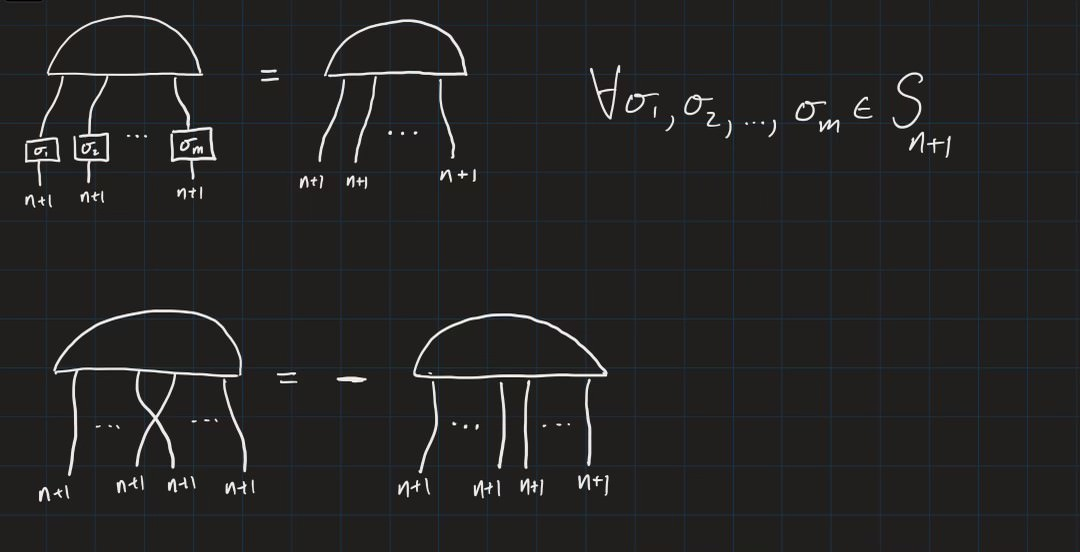
\includegraphics[scale=0.25]{Symm.jpg}\]
\end{itemize}
The first goal is to find a rule for $\phi$. The rule is given by the determinant in the case $n=0$. I gave the rule for $\mathfrak{sosp}(1|2)$ at the start of the Spring 2024 independent study, and we found the rule for $\mathfrak{sosp}(2|2)$ at the end of that independent study. What is the rule for arbitrary $m$ and $n$?

\subsection{Find the jellyfish relation}

Stacking a jellyfish under an upside-down jellyfish gives us a map $V^{\otimes m(n+1)}\to V^{\otimes m(n+1)}$. The rule for this map is completely determined by $\phi$. I expect this map can be realized as a linear combination of Brauer diagrams (without jellyfish). The goal here is to explain how to write this map as linear combo of Brauer diagrams. 


\vfill


\end{document}

